\documentclass[aspectratio=169]{beamer}
\usetheme{Madrid}
\usecolortheme{seahorse}

\usepackage{fontenc}
\usepackage{graphicx}

\title{\textbf{myOCW}}
\subtitle{Giving OpenCourseWare a facelift!}
\author{}
\date{}

\setbeamertemplate{navigation symbols}{}
\setbeamertemplate{footline}{}

\begin{document}

\begin{frame}
\titlepage
\end{frame}

\begin{frame}{Starting Point}
\centering
\Large
OCW is one of the most important\\
educational projects ever made.\\[2em]
\normalsize
We wanted to explore what new tools\\
could add on top of that foundation.
\end{frame}

\begin{frame}{What is myOCW?}
\centering
\Large
A companion layer built on OCW content.\\[0.5em]
\normalsize
Building this led to some other cool stuff!\\[0.5em]
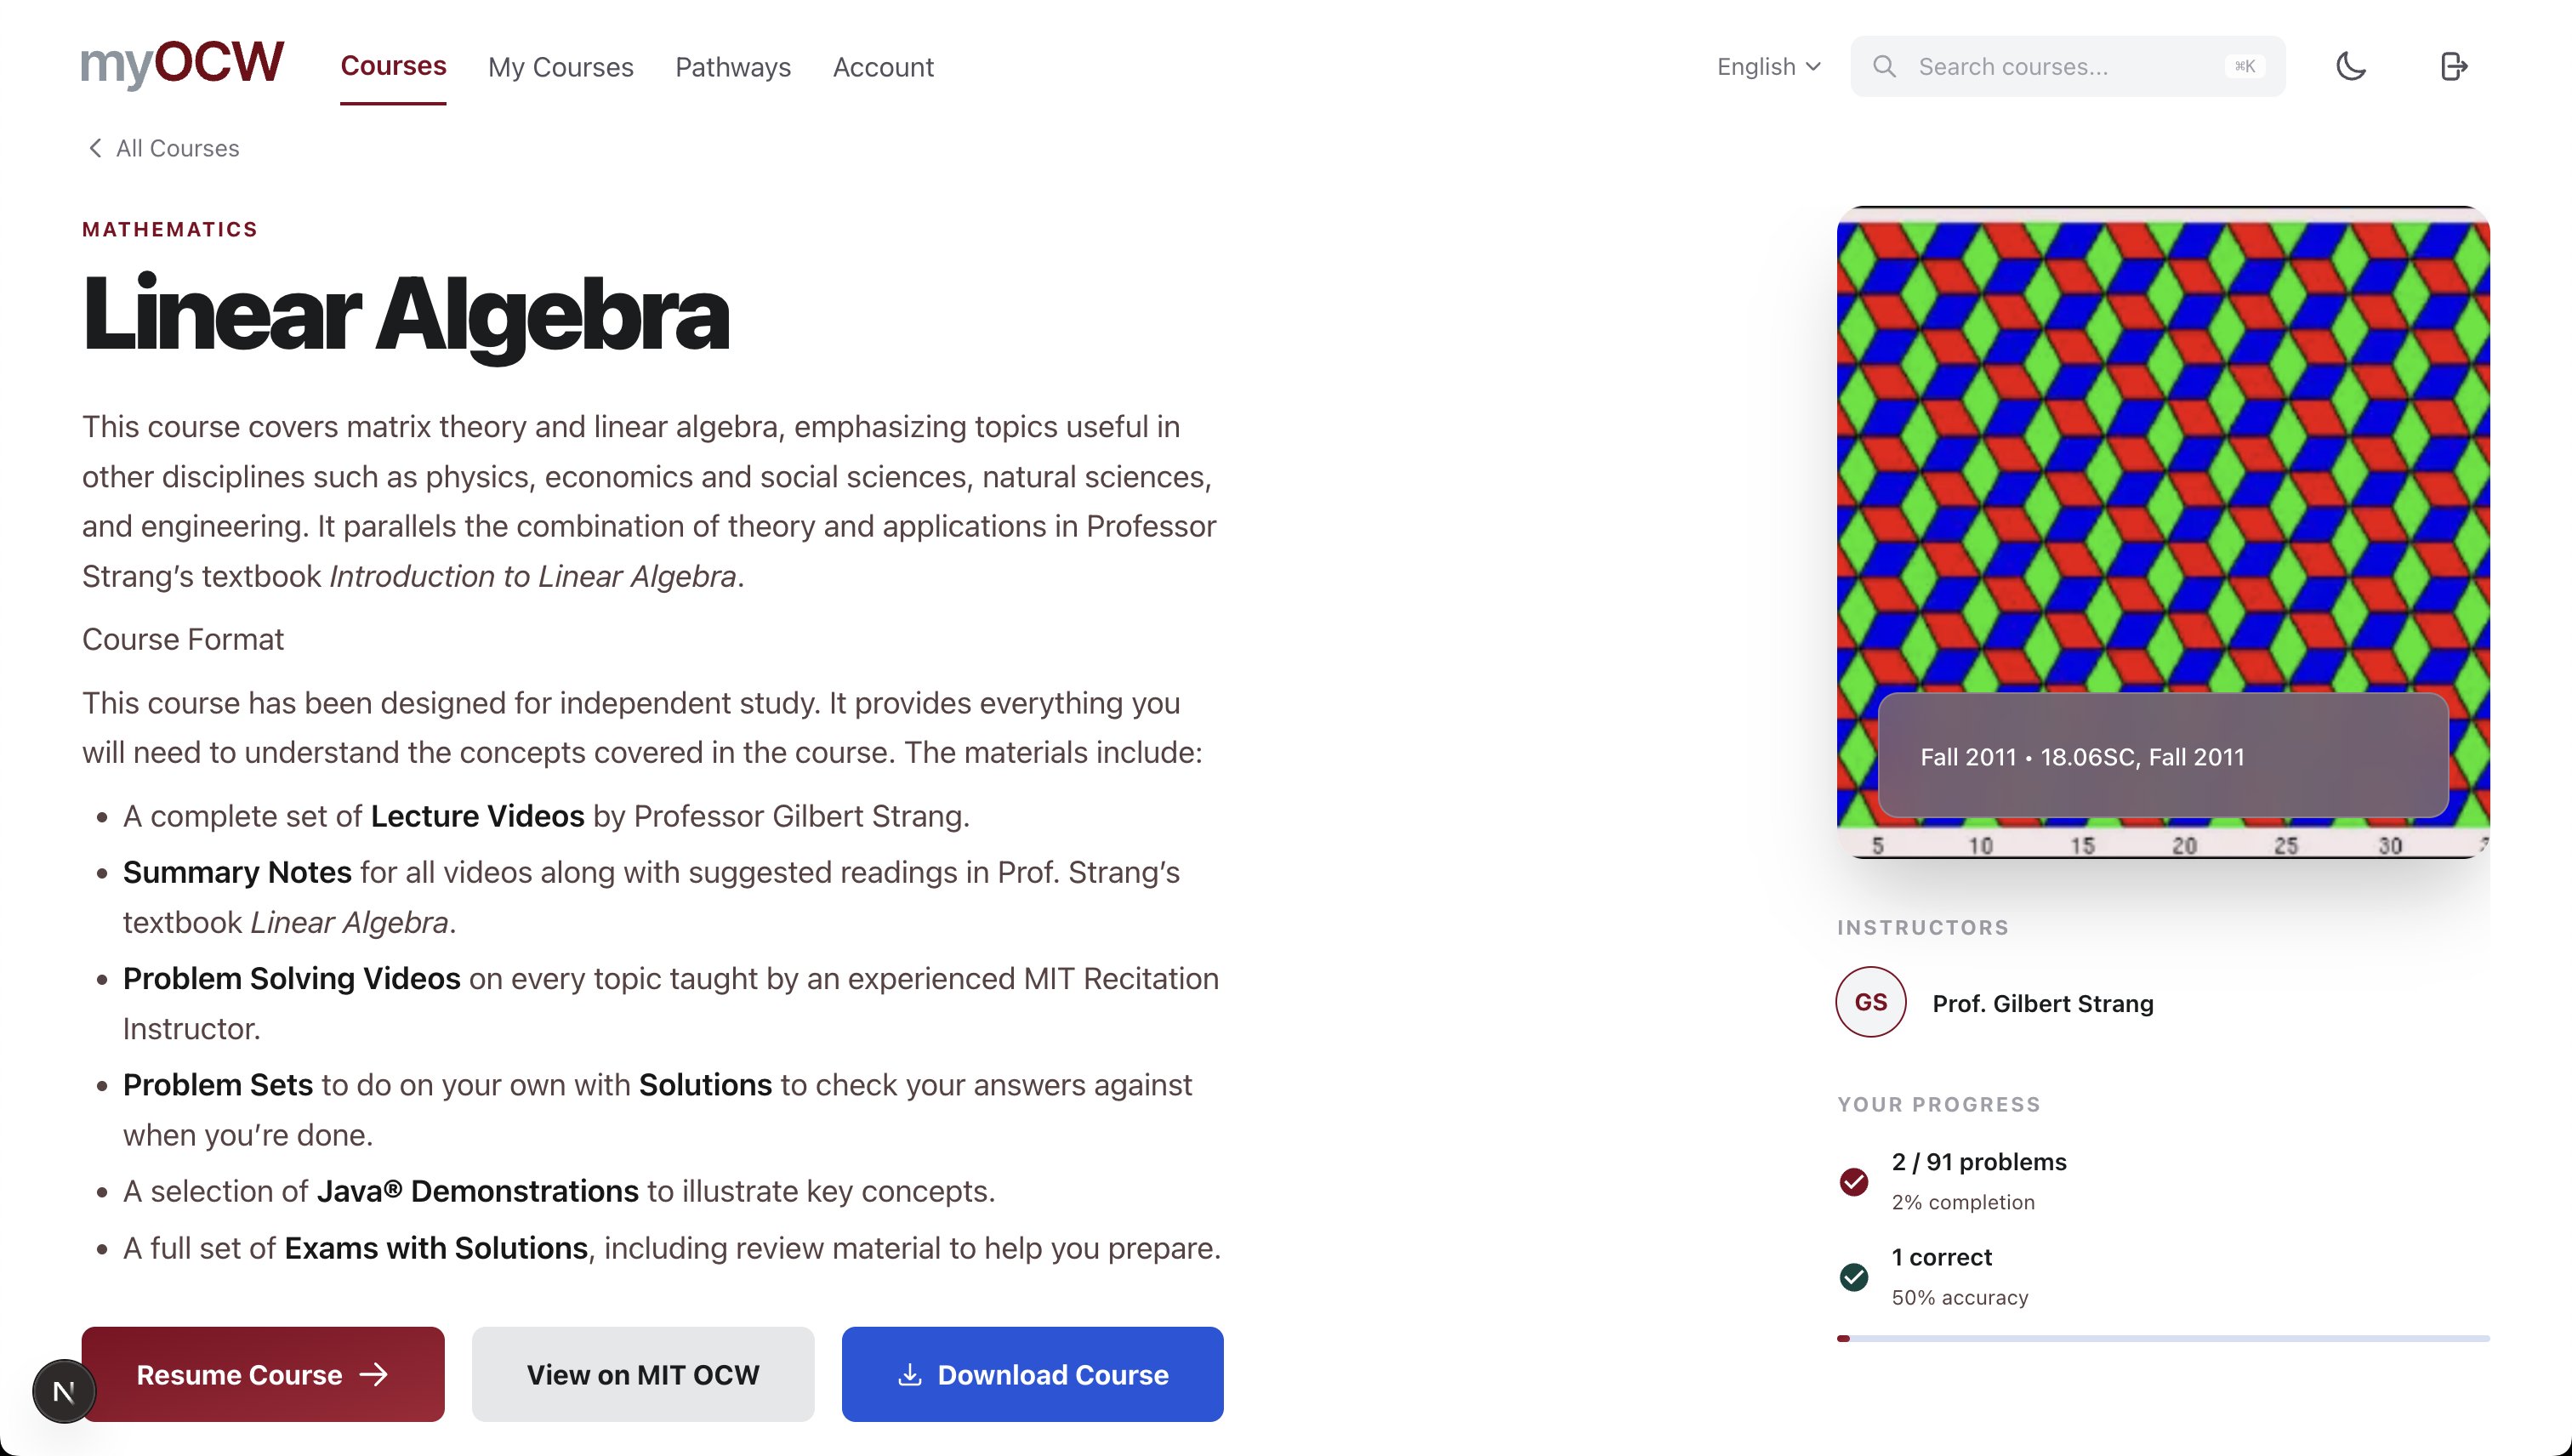
\includegraphics[width=0.7\textwidth]{public/courseheader.png}
\end{frame}

\begin{frame}{Compression: PDFs}
\begin{columns}
\begin{column}{0.45\textwidth}
\centering
\Large
PDF $\rightarrow$ Markup\\[0.5em]
\normalsize
Gil Strang's Linear Algebra:\\[0.3em]
\Large
\textbf{50 MB $\rightarrow$ 1.5 MB}\\[0.3em]
\normalsize
$\sim$97\% reduction
\end{column}
\begin{column}{0.55\textwidth}
\centering
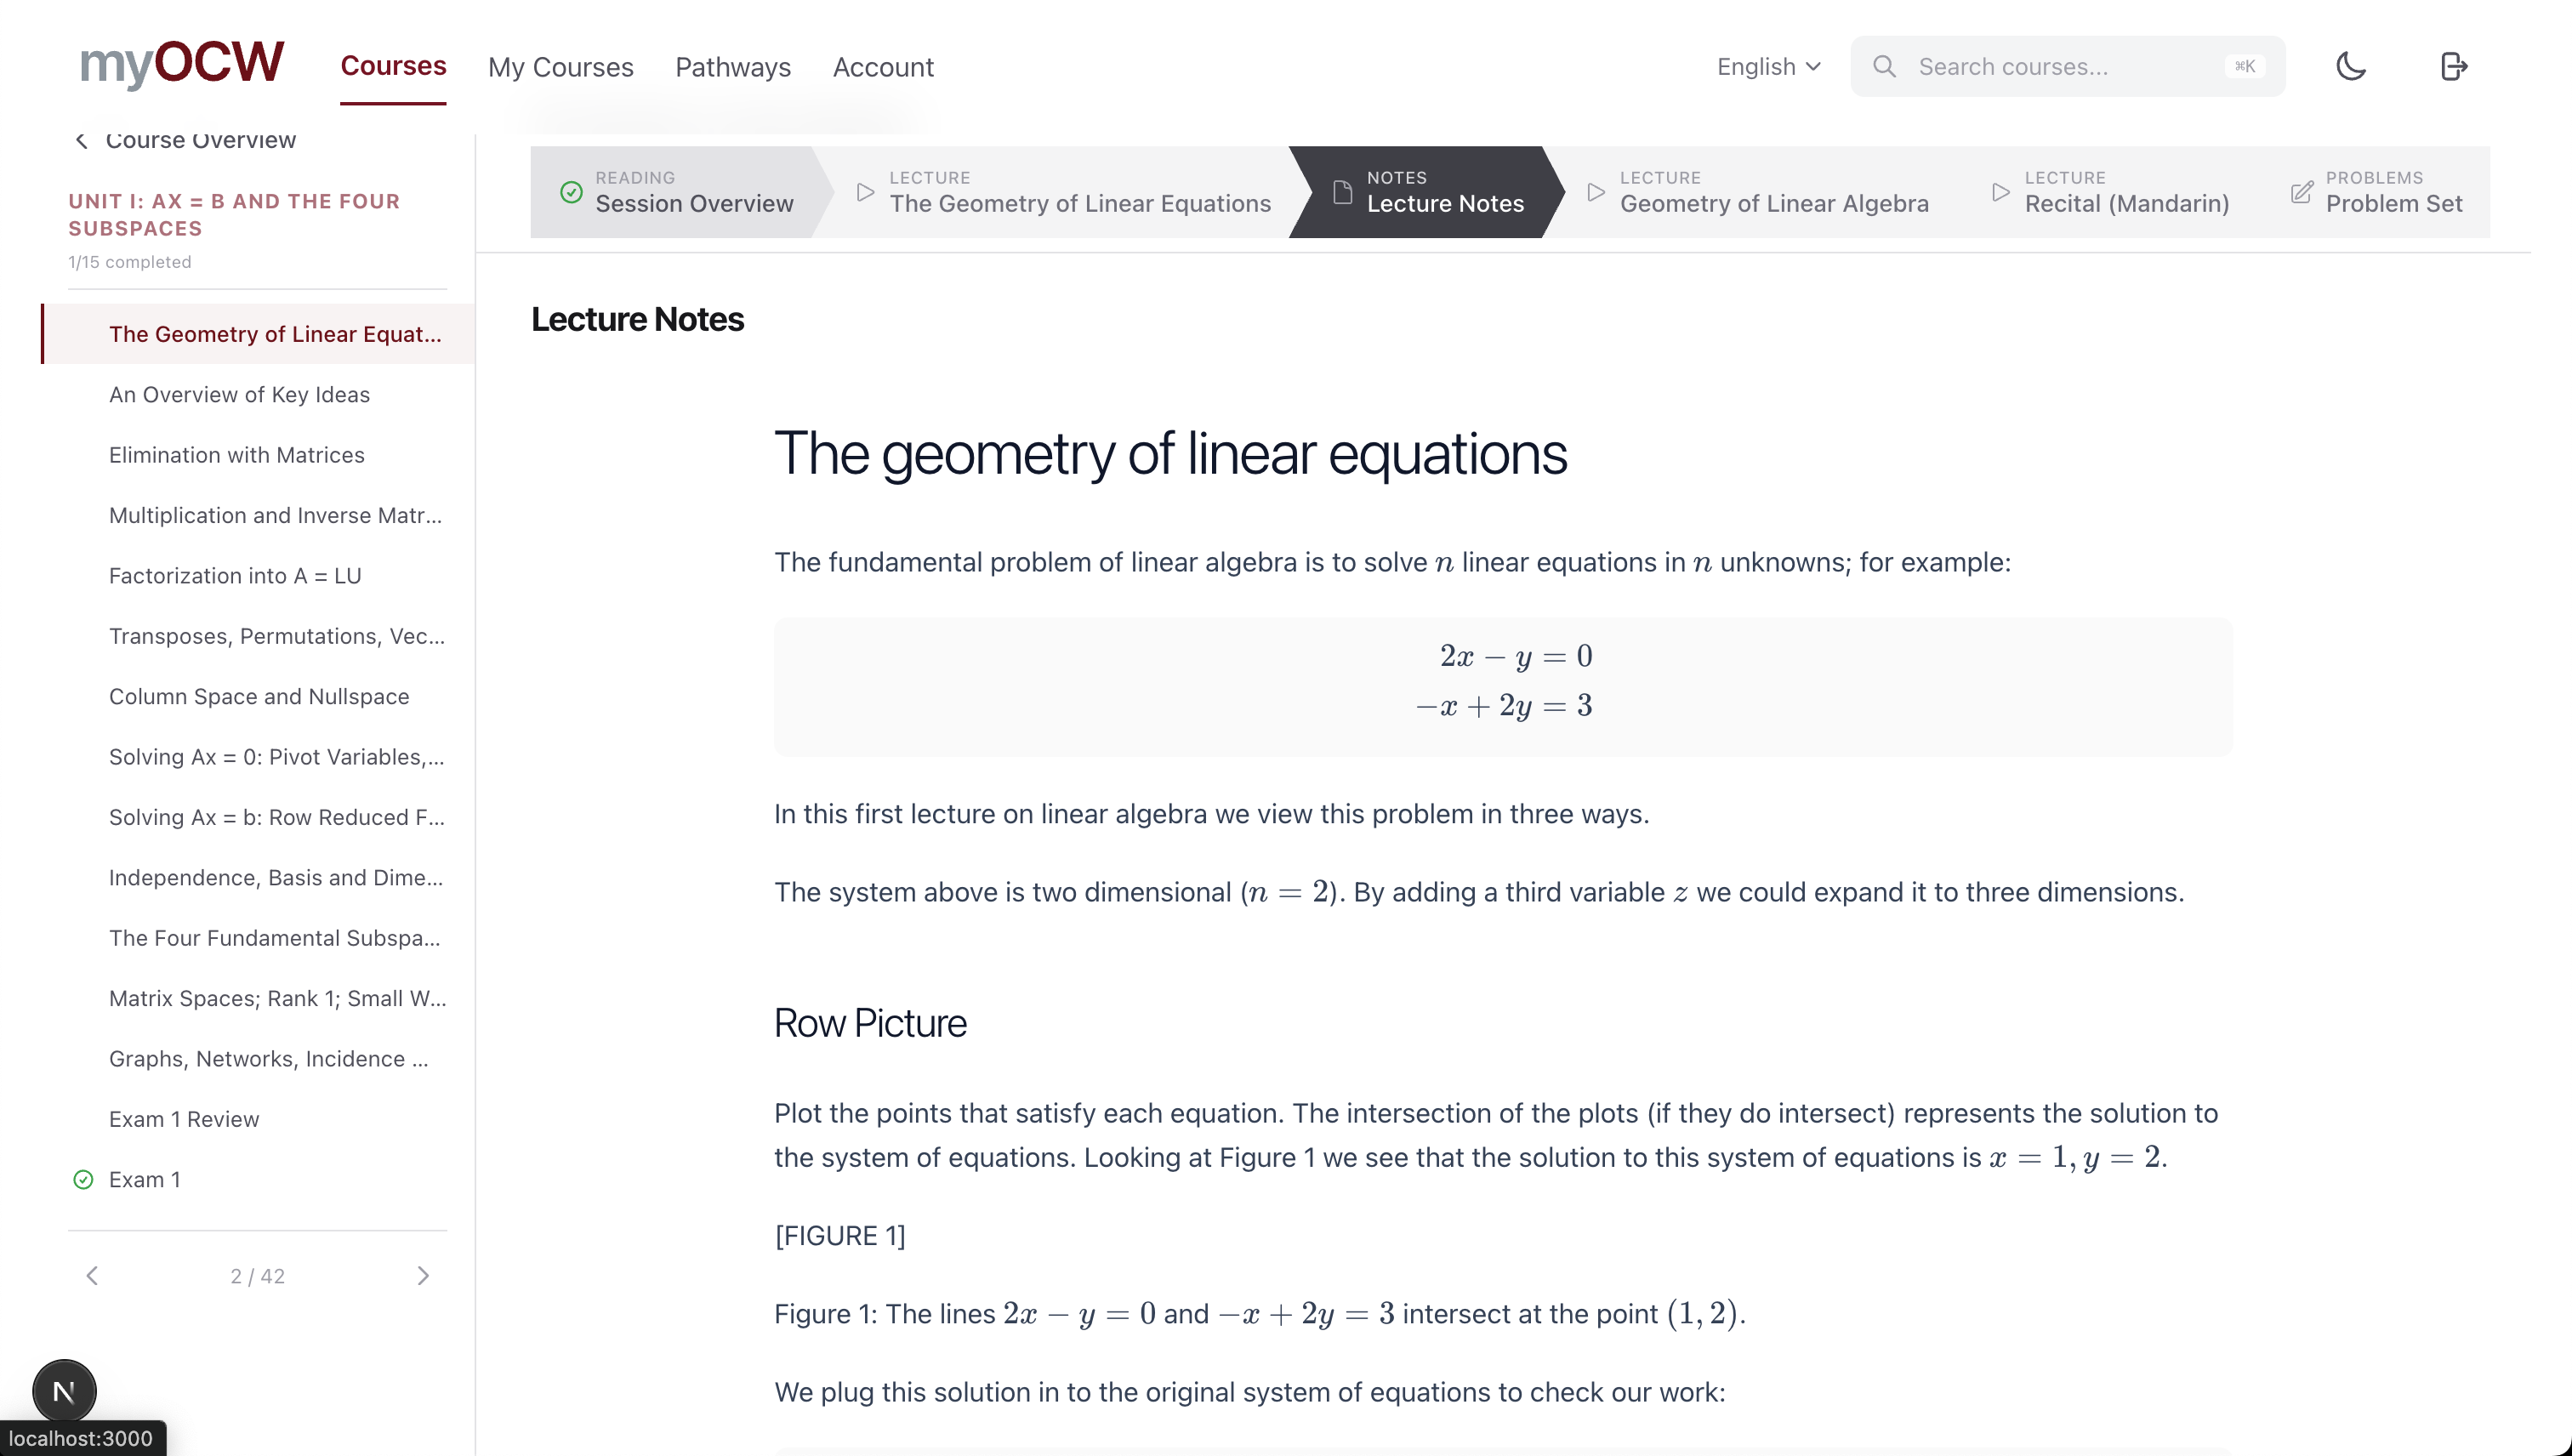
\includegraphics[width=\textwidth]{public/lecturenotesdemo.png}
\end{column}
\end{columns}
\end{frame}

\begin{frame}{Compression: Video}
\centering
\Large
Lecture video compression techniques we tried:\\[1em]
\normalsize
Lower framerate in static regions.\\
Reducing resolution outside the blackboard area.\\
\textbf{50-70\% filesize reduction}, minimal quality loss.\\
Up to \textbf{90\%} may be achievable.
\end{frame}

\begin{frame}{Interactive Problem Sets}
\begin{columns}
\begin{column}{0.4\textwidth}
\Large
Parsed problems from PDFs\\
into interactive cards.\\[0.5em]
\normalsize
Students answer in-app\\
and check solutions\\
one at a time.
\end{column}
\begin{column}{0.6\textwidth}
\centering
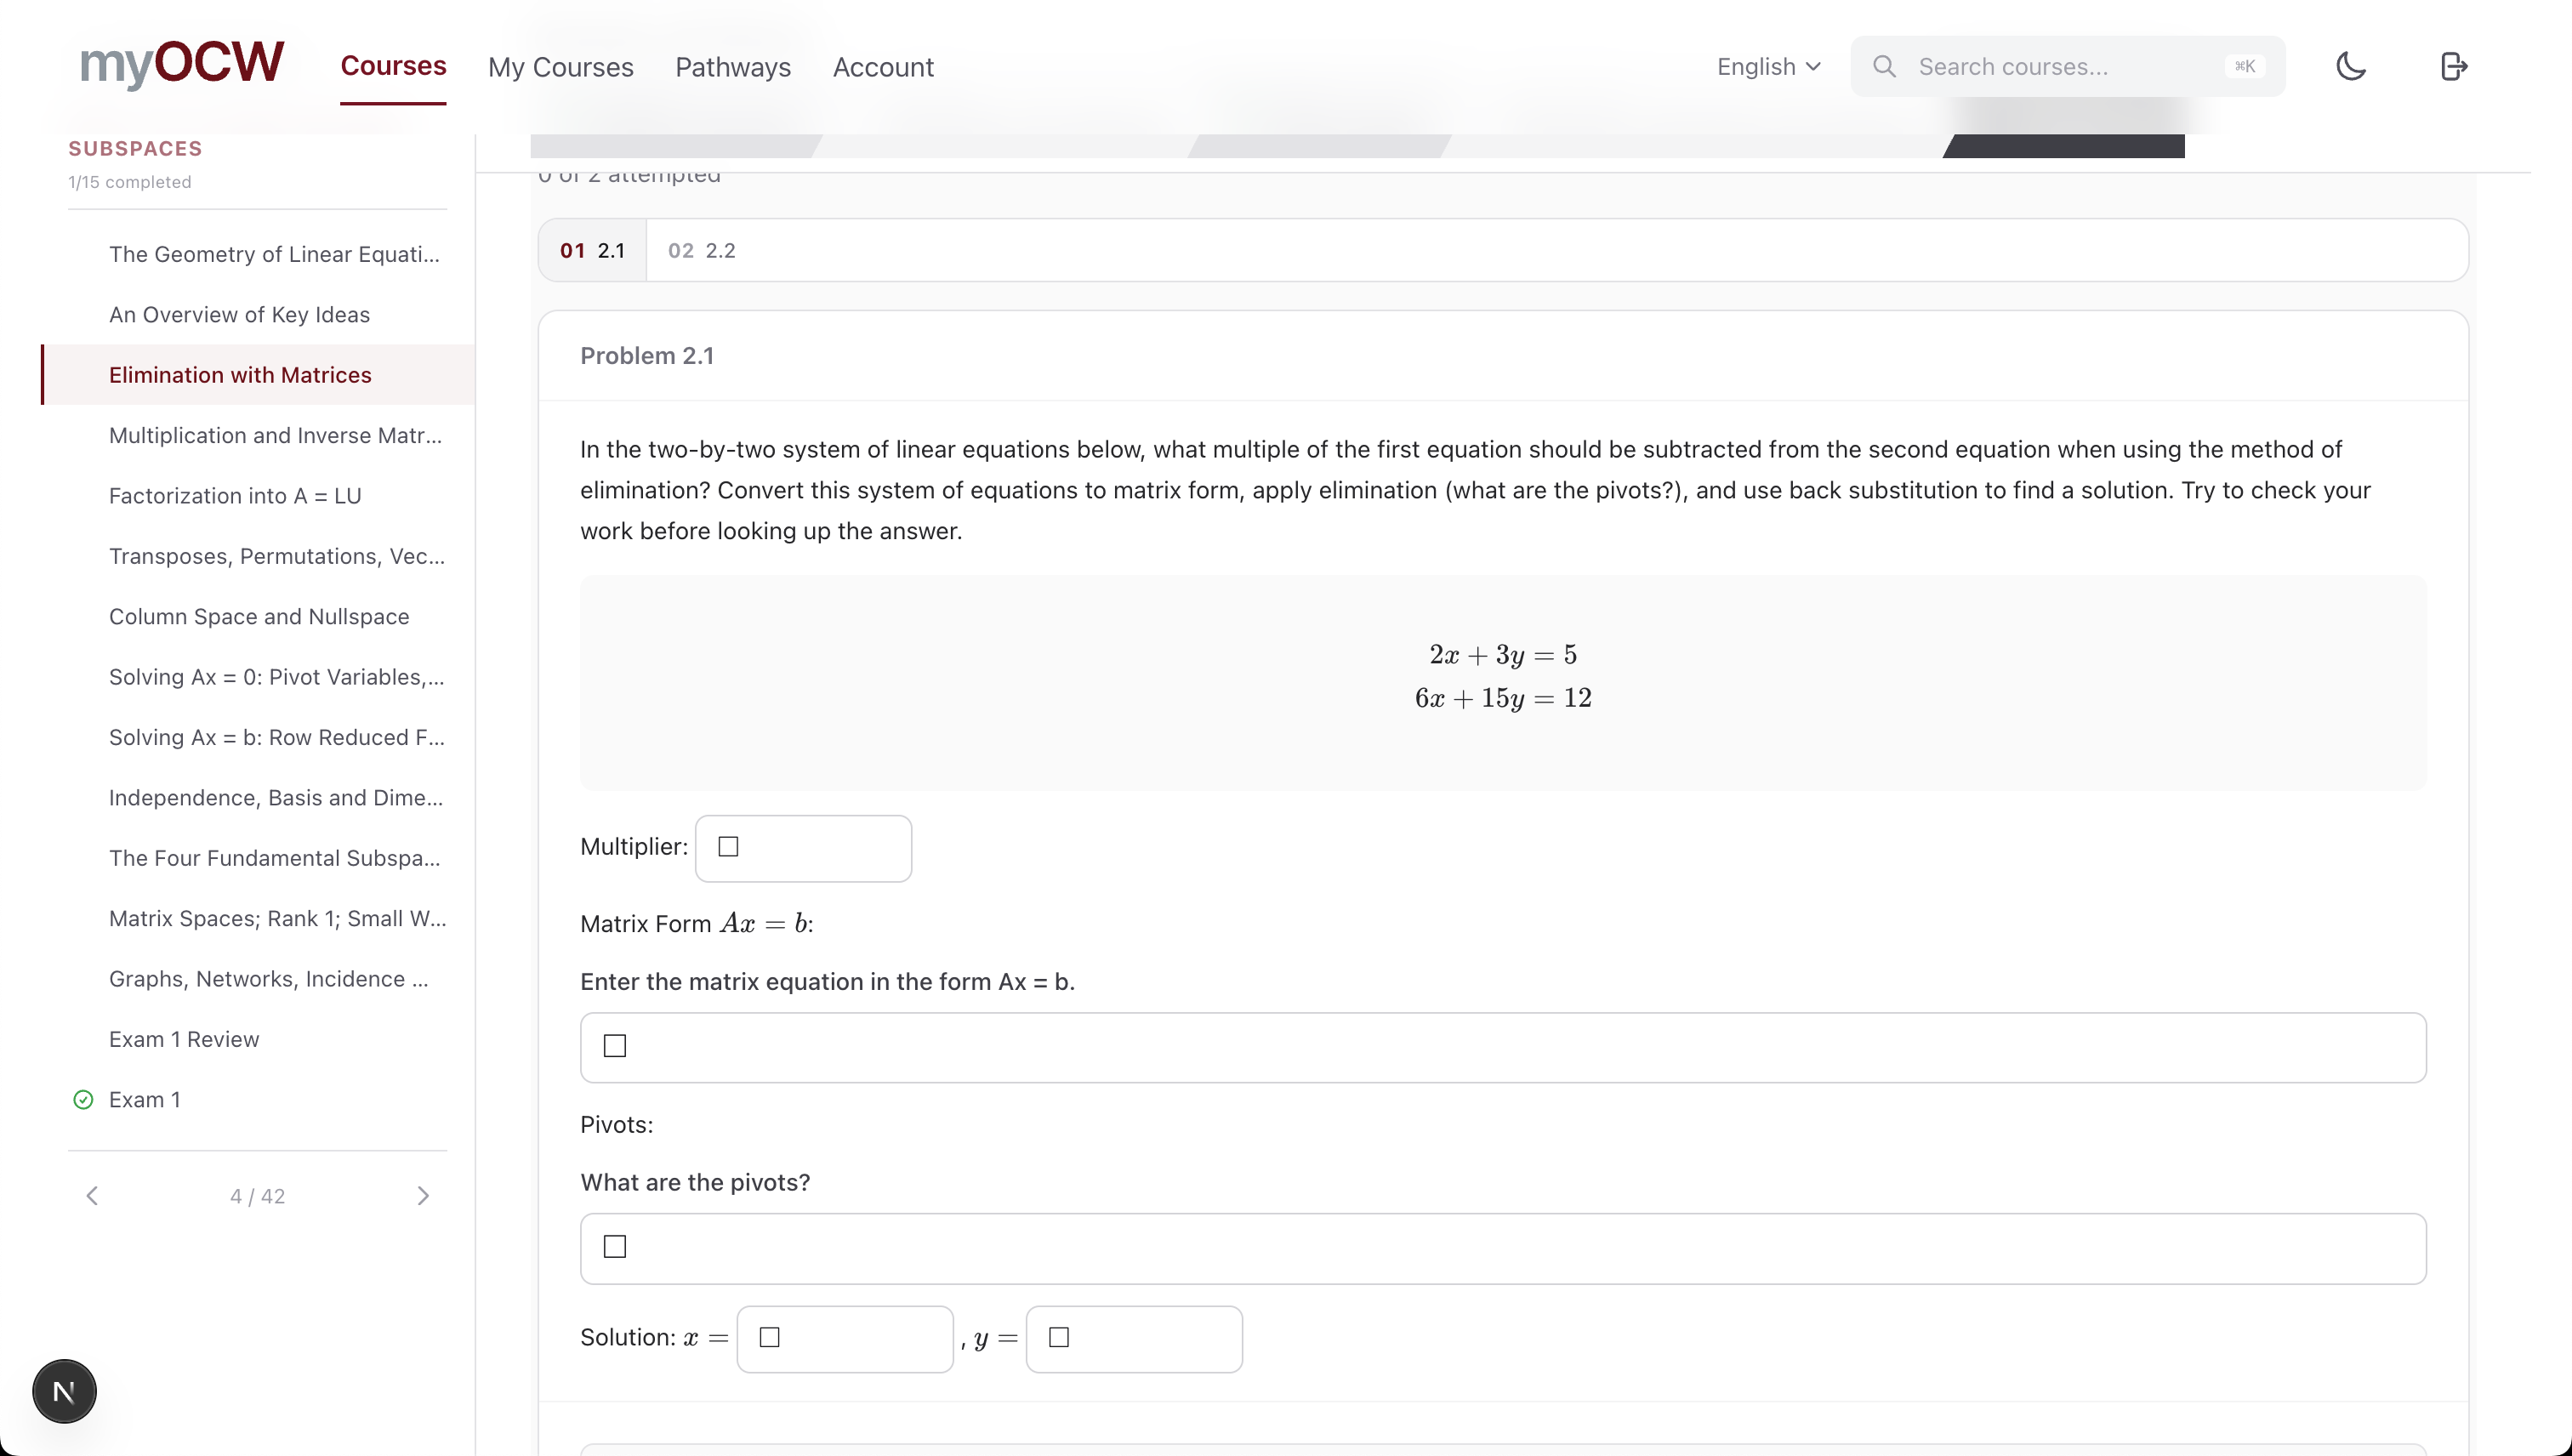
\includegraphics[width=\textwidth]{public/psetdemo.png}
\end{column}
\end{columns}
\end{frame}

\begin{frame}{Machine Translation}
\centering
\Large
Markup makes translation straightforward.\\[1em]
\normalsize
PDF $\rightarrow$ Markup $\rightarrow$ LLM $\rightarrow$ Any language\\[1.5em]
\normalsize
A path to making OCW courses\\
accessible to non-English speakers worldwide.
\end{frame}

\begin{frame}{Accounts: Optional, Minimal}
\centering
\Large
No login required to use the platform.\\[1em]
\normalsize
Optional signup with just name + password.\\
No email needed. Minimal bandwidth overhead.\\[1.5em]
Enables progress tracking and learning analytics.
\end{frame}

\begin{frame}{Conversion Cost}
\centering
\Large
\textbf{\$1--3, 1hr per course}\\[0.5em]
\normalsize
to convert PDF materials to interactive markup.\\[2em]
\Large
2,580 courses in the OCW catalog.\\[0.3em]
\normalsize
Estimated full conversion: \$3K--8K.
\end{frame}

\begin{frame}{Sustainability}
\centering
\Large
Core platform: free\\[1.5em]
\normalsize
One possibility for monetization: AI-powered study insights\\
as a perk for donors or supporters.\\[1em]
Very early thinking on this front.
\end{frame}

\begin{frame}{}
\centering
\Huge
\textbf{myOCW}\\[1em]
\Large
name is a WIP!\\[2em]
\normalsize
Also: OCW Mobile App!
\end{frame}

\end{document}
